\documentclass[12pt,a4paper]{article}

\usepackage[utf8]{inputenc}
\usepackage[T1]{fontenc}
\usepackage{graphicx}
\usepackage{hyperref}
\usepackage{geometry}
\usepackage{chngcntr}
\usepackage{setspace}
\usepackage{datetime}
\usepackage{booktabs}
\usepackage{tabularx}
\usepackage{longtable}
\usepackage{enumitem}
\usepackage{tikz}
\usepackage{listings}
\usepackage{xcolor}
\usepackage{url}
\usepackage{amsmath}

\usetikzlibrary{arrows.meta,positioning}
\geometry{a4paper,inner=1in,outer=1in,bindingoffset=.5cm,top=.75in,bottom=.75in}
\setstretch{1.35}
\counterwithin{table}{section}
\counterwithin{figure}{section}
\hypersetup{colorlinks=true,linkcolor=blue,citecolor=blue,urlcolor=blue}
\newdateformat{monthyeardate}{\monthname[\THEMONTH], \THEYEAR}
\newcommand{\HRule}{\rule{.9\linewidth}{.6pt}}
\newcommand{\myemptypage}{\null\thispagestyle{empty}\newpage}

\newcommand{\ttitle}{TenderWorks: An Evidence-Backed Concept Estimation Workspace for Government Works}
\newcommand{\authorname}{[Student Name]}
\newcommand{\rn}{[Roll Number]}
\newcommand{\supname}{[Supervisor Name]}
\newcommand{\degree}{B.Tech. Project}
\newcommand{\univname}{Indian Institute of Technology Jodhpur}
\newcommand{\deptname}{[Department Name]}

\begin{document}
\begin{titlepage}
\begin{center}
\vspace*{1.1cm}
{\Huge\bfseries \ttitle\par}
\vspace{2.0cm}
{\Large A Project Report Submitted by\par}
\vspace{0.6cm}
{\LARGE\bfseries \authorname\par}
\vspace{0.2cm}
{\large Roll No.: \rn\par}
\vfill
{\Large in partial fulfilment of the requirements for\par}
\vspace{0.3cm}
{\Large\bfseries \degree\par}
\vfill
\IfFileExists{IITJlogo.png}{
\includegraphics[width=0.25\textwidth]{IITJlogo.png}\par\vspace{0.8cm}}{}
{\Large\bfseries \univname\par}
\vspace{0.2cm}
{\large \deptname\par}
\vspace{0.8cm}
{\large Supervisor: \supname\par}
\vspace{0.5cm}
{\large\monthyeardate\today\par}
\end{center}
\end{titlepage}

\pagenumbering{roman}
\setcounter{page}{1}
\section*{Declaration}
\addcontentsline{toc}{section}{Declaration}
I hereby declare that this report, titled \emph{\ttitle}, is an account of the project work carried out by me under the supervision of \supname. The work presented here is based on the Tenderworks software project and the sources identified in this report. To the best of my knowledge, this report has not been submitted, in whole or in part, to another institute or university for an academic award.

\vspace{2cm}
\begin{flushright}
\textbf{Signature}\\[0.4cm]
\authorname\\
Roll No.: \rn
\end{flushright}
\clearpage

\section*{Certificate}
\addcontentsline{toc}{section}{Certificate}
This is to certify that the project report titled \emph{\ttitle}, submitted by \authorname{} (Roll No. \rn) to \univname{} in partial fulfilment of the requirements for the \degree, is a record of project work carried out under my supervision.

\vspace{2cm}
\begin{flushright}
\textbf{Signature of Supervisor}\\[0.5cm]
\supname\\
\deptname
\end{flushright}
\clearpage

\section*{Acknowledgements}
\addcontentsline{toc}{section}{Acknowledgements}
I would like to express my gratitude to my project supervisor, \supname, for guidance and feedback during this work. I also acknowledge the faculty and staff of \univname{} and everyone who contributed advice or feedback to the development and evaluation of TenderWorks.

\vspace{1cm}
\begin{flushright}
\authorname
\end{flushright}
\clearpage

\section*{Abstract}
\addcontentsline{toc}{section}{Abstract}
Preparing an early-stage works estimate from a project brief requires a consistent scope, defensible quantities, applicable rates, and traceable evidence. TenderWorks is a prototype workspace that turns a structured building brief and a reviewed domain package into a concept design, quantity schedule, priced bill of quantities (BOQ), and supporting report. Its web application combines incremental source-document ingestion, a persistent workflow, deterministic geometry and decimal arithmetic, and optional language-model assistance.

The workflow is organized into three checkpoints. It first routes a brief to an applicable package, plans scope, creates supported rectangular-building concept geometry, computes quantities, and verifies coverage. It then matches exact component specifications, units, and effective dates to scheduled or resource-built rates and calculates amounts using decimal arithmetic. Finally, it audits evidence and calculation links before compiling exportable artifacts. Retrieved passages and model findings are advisory; they do not supply quantities, rates, or totals. Unsupported inputs remain visible as unresolved items rather than being silently assigned zero.

The implementation provides a FastAPI workspace, persistent LangGraph checkpoints, tenant-scoped relational storage, content-addressed source snapshots, and PDF, XLSX, DOCX, SVG, DXF, and JSON exports. The bundled domain examples and reference cases use synthetic data. The automated test suite completed with 36 passing tests during preparation of this report. This demonstrates tested software behavior, not real-world price or engineering accuracy. TenderWorks is an estimating aid for concept-stage review, not a sanctioned estimate, construction design, or tender publication system.

\noindent\textbf{Keywords:} tender estimation, bill of quantities, quantity take-off, evidence provenance, retrieval-augmented generation, deterministic calculation, human review
\clearpage

\tableofcontents
\clearpage
\listoffigures
\listoftables
\clearpage
\pagenumbering{arabic}
\section{Introduction}
\subsection{Project context}
Public works estimates combine project requirements, quantity measurement, applicable schedule rates, and administrative rules. At the concept stage, the brief is often incomplete and source material may span revisions, document formats, and jurisdictions. A spreadsheet can record a total, but it does not by itself establish which brief facts drove the design, how a quantity was derived, or which source row supports a selected rate.

TenderWorks is a local-first software prototype for preparing evidence-linked, concept-stage estimates for configured government building packages. The intended flow is: enter a project brief, create and review a supported concept, calculate quantities, select applicable rates, audit the resulting evidence, and export a draft BOQ and report. The software is designed to expose assumptions and uncertainty instead of implying that a preliminary estimate is final.

\subsection{Problem statement}
The central problem addressed is how to make early works estimates reproducible and reviewable when source data, geometry, and applicability rules must be managed together. A useful system must connect every amount to its quantity calculation and rate source, preserve the source version used, and distinguish a complete estimate from a known subtotal with unresolved items.

\subsection{Objectives}
\begin{enumerate}[leftmargin=*]
  \item Provide an end-to-end web workflow from a structured project brief to a draft BOQ.
  \item Ingest source documents incrementally while preserving their versions and locators.
  \item Use explicit package rules and deterministic engines for geometry, measurements, and costs.
  \item Keep optional language-model and retrieval features bounded, advisory, and reviewable.
  \item Verify scope, arithmetic, and evidence before compiling reports and other deliverables.
  \item Make limitations and unresolved work visible to the user.
\end{enumerate}

\subsection{Contributions}
The project integrates five capabilities in one prototype: (i) version-aware source ingestion and package governance; (ii) a persistent three-checkpoint estimation workflow; (iii) structured concept geometry with measurement recipes; (iv) exact rate matching and decimal cost calculations; and (v) a traceable evidence chain included in generated exports. Its contribution is a software workflow and its controls; it does not establish a new civil-engineering measurement standard.

\subsection{Scope}
The bundled concept templates are limited to rectangular layouts for schools, offices, and community halls. Foundations, reinforcement, and service-capacity quantities may be explicit template allowances until engineering inputs are supplied. Government rates, source schedules, mappings, and reference estimates are not bundled as authoritative data. Actual use therefore depends on verified, approved domain packages and qualified professional review.

\section{Background and Related Work}
\subsection{Document retrieval and estimation evidence}
Retrieval-augmented generation (RAG) combines a language model with retrieved external passages to ground responses in a knowledge collection \cite{lewis2020rag}. TenderWorks uses retrieval as a discovery and review aid: passages can be indexed and surfaced with source locators, but they are not treated as numeric calculation inputs. This boundary is important because textual similarity alone does not establish that a schedule rate is legally or technically applicable.

The local retrieval mode ranks indexed text with keyword matching; optional embeddings add semantic candidates to a hybrid retrieval path. The ingestion guide describes tenant, authority, location, and date filtering, alongside bounded chunks and source-version retention \cite{tenderworks2026}. A BM25-style keyword ranker is a conventional retrieval baseline \cite{robertson2009bm25}; the software's use of retrieval does not by itself establish a quality advantage over that baseline.

\subsection{Workflow orchestration and deterministic computation}
Graph-based orchestration is useful when a process has explicit state, conditional routes, retries, and human review. TenderWorks uses LangGraph checkpoints to persist workflow state and to resume a revision after a review interrupt \cite{langgraphDocs}. Pydantic contracts validate the structured brief, domain package, design revision, BOQ, and evidence records. The geometry and pricing engines remain deterministic: model output cannot override those calculations \cite{tenderworks2026}.

\subsection{Gap addressed}
The prototype addresses the gap between a free-text brief and an auditable draft estimate by joining document provenance, scope, geometry, quantities, and prices in a revision-specific record. It does not automate the professional judgment needed to approve source mappings, design assumptions, or legal applicability.

\section{Requirements and System Design}
\subsection{Users and requirements}
The system distinguishes engineer, viewer, reviewer, and administrator roles. Engineers can prepare and revise estimates; viewers have read-only access; reviewers can make review decisions; and administrators manage package approval. The server enforces tenant and role boundaries. The default local demonstration mode is intended for a trusted local user rather than an exposed deployment.

\begin{table}[htbp]
\centering
\caption{Core requirements and implementation approach}
\label{tab:requirements}
\begin{tabularx}{\textwidth}{p{0.24\textwidth}X}
\toprule
\textbf{Requirement} & \textbf{Implementation approach}\\
\midrule
Traceable quantities and prices & Store calculation records, evidence IDs, source locators, and assumptions with each revision.\\
Safe treatment of missing data & Preserve unresolved BOQ lines and report a known subtotal rather than a false complete total.\\
Reproducible source use & Snapshot source documents, retain hashes and versions, and pin the selected package to each revision.\\
Reliable calculations & Use reviewed measurement expressions and Python \texttt{Decimal} arithmetic; do not delegate arithmetic to a model.\\
Reviewable automation & Persist workflow stages, expose findings, and support explicit review interruptions and new revisions.\\
Usable deliverables & Compile the estimate and its supporting evidence into downloadable report and data formats.\\
\bottomrule
\end{tabularx}
\end{table}

\subsection{High-level architecture}
The application is a FastAPI service with a browser workspace and JSON APIs. SQLAlchemy stores relational project, revision, source, package, review, and feedback records. LangGraph persists workflow checkpoints in SQLite for local use or PostgreSQL for a configured deployment. Source snapshots and generated artifacts are stored by content-addressed object keys. A knowledge gateway supports keyword retrieval and optional hybrid retrieval. These components and their contracts are described in the project's architecture document \cite{tenderworks2026}.

\begin{figure}[htbp]
\centering
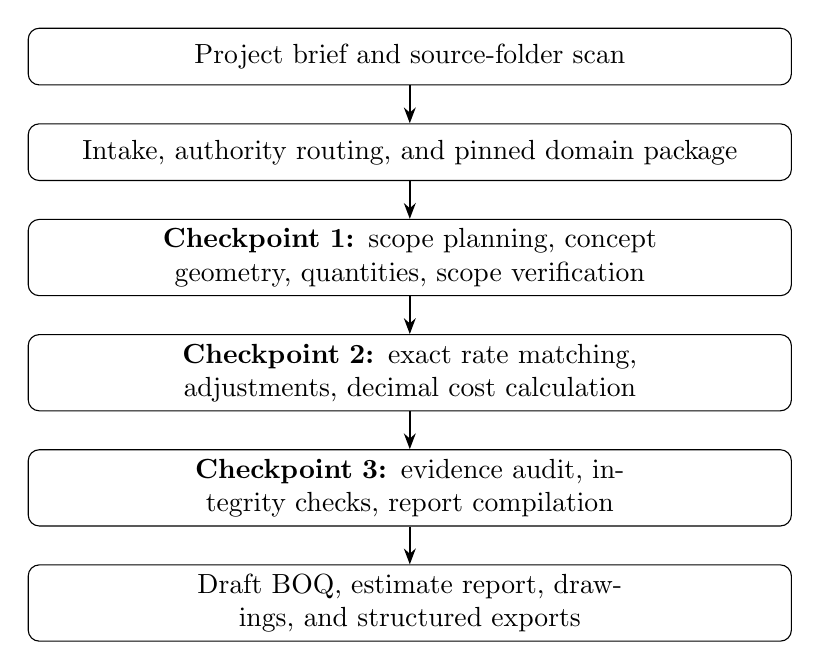
\begin{tikzpicture}[
  node distance=0.48cm,
  stage/.style={draw,rounded corners,align=center,text width=0.78\textwidth,minimum height=0.72cm},
  arrow/.style={-{Stealth[length=2mm]},thick}
]
\node[stage] (brief) {Project brief and source-folder scan};
\node[stage,below=of brief] (route) {Intake, authority routing, and pinned domain package};
\node[stage,below=of route] (cp1) {\textbf{Checkpoint 1:} scope planning, concept geometry, quantities, scope verification};
\node[stage,below=of cp1] (cp2) {\textbf{Checkpoint 2:} exact rate matching, adjustments, decimal cost calculation};
\node[stage,below=of cp2] (cp3) {\textbf{Checkpoint 3:} evidence audit, integrity checks, report compilation};
\node[stage,below=of cp3] (out) {Draft BOQ, estimate report, drawings, and structured exports};
\draw[arrow] (brief) -- (route);
\draw[arrow] (route) -- (cp1);
\draw[arrow] (cp1) -- (cp2);
\draw[arrow] (cp2) -- (cp3);
\draw[arrow] (cp3) -- (out);
\end{tikzpicture}
\caption{Simplified TenderWorks estimate lifecycle. Optional retrieval and specialist review supplement, but do not replace, deterministic computation.}
\label{fig:workflow}
\end{figure}

\subsection{Data contracts and provenance}
The core contracts include \texttt{ProjectBrief}, \texttt{DomainPack}, \texttt{DesignRevision}, \texttt{BOQItem}, \texttt{EvidenceRecord}, and \texttt{CalculationRecord}. Quantities and amounts are serialized as decimal strings. Evidence records refer to source snapshots, versions, hashes, and locators; calculation records refer to the evidence and inputs used.

The intended provenance chain is:
\[
\text{amount} \longrightarrow \text{quantity calculation and rate}
\longrightarrow \text{design model, source snapshot, and assumptions}.
\]
Each estimate revision pins a package snapshot so that later package changes do not silently rewrite an earlier result.

\section{Source Ingestion and Knowledge Management}
\subsection{Incremental ingestion}
The \texttt{database/} folder is the document inbox. Supported input formats include PDF, DOCX, text/Markdown, CSV, XLSX, and JSON. For each file, the ingestor hashes its bytes together with any metadata sidecar. Unchanged versions are skipped; new or changed files are extracted, snapshotted, chunked, and indexed. Failed extractions remain visible and are retried. A scanned PDF without a usable text layer is not treated as if its content had been read \cite{tenderworks2026}.

Extracted records preserve useful structural locators such as PDF pages, document tables, spreadsheet headers, and row numbers. Older versions remain available for historical estimates, while the current inbox version is the default retrieval candidate.

\subsection{Domain packages and authority}
Searchable documents and approved numeric rate records are separate. A domain package binds a reviewed authority, region, work category, effective period, source documents, component specifications, units, measurement recipes, rates, and applicable rules. Package imports enter candidate status and require administrative review. The rate engine selects a record by the complete specification, unit, and effective date rather than by a loosely similar description.

\subsection{Optional retrieval and specialist assistance}
Local operation uses keyword retrieval and deterministic templates without requiring credentials. Optional embedding, NVIDIA RAG, Anthropic, or public-source research capabilities require explicit configuration. Retrieved text is advisory and is stored as retrieved evidence. A model-generated review must cite a retrieved evidence identifier and an exact quote from that passage; even a valid finding cannot directly change quantities, rates, or totals. If a provider is unavailable, the application identifies local template/rule operation rather than claiming that semantic retrieval occurred.

\section{Estimation Methodology}
\subsection{Checkpoint 1: brief, scope, and concept quantities}
The first checkpoint extracts explicit brief facts and routes the project to a package. Rules and a scope planner identify components. The geometry engine then constructs a supported rectangular concept from supplied dimensions or from configured defaults. It records inferred dimensions and template assumptions, and rejects unsupported dimensions or building forms rather than extrapolating beyond its template.

Each package measurement recipe uses named geometry metrics and a small arithmetic language. The expression evaluator accepts names, decimal numbers, addition, subtraction, multiplication, division, unary minus, and parentheses; it does not execute arbitrary Python, function calls, or attribute access. Quantities are rounded to the nearest \(0.001\) unit for measurement. Supplied quantities can override a recipe while retaining their user-input provenance.

\subsection{Checkpoint 2: rate selection and costing}
For each component, the workflow matches the exact specification and unit against applicable, unsuperseded rate records for the estimate date. Conflicting matches remain unresolved. Non-scheduled rates can be assembled from individually sourced resources; unsupported resources do not receive invented prices.

For item \(i\), a priced line is calculated as
\[
A_i = \operatorname{round}_{0.01}(Q_i R_i),
\]
where \(Q_i\) is the accepted quantity, \(R_i\) is the selected unit rate, and the monetary rounding uses decimal arithmetic. Eligible, sourced adjustments are added only to their explicitly defined bases; overlapping adjustment groups and duplicate inclusions are checked. Scenario, optional-item, and unresolved-line totals remain distinguishable.

\subsection{Checkpoint 3: audit and report}
Before compilation, the workflow checks that required evidence and calculation references exist and that stored source objects match their recorded hashes. Blocking findings prevent an unsupported complete estimate. A missing required rate or quantity can yield an incomplete report with its known subtotal and unresolved lines. The compiler builds reports and BOQs from the validated estimate records rather than from free-form model text.

\subsection{Revision and human-review behavior}
An optional design-review interrupt is persisted and can be resumed after explicit acceptance. Changes are made as new revisions, recomputing geometry, quantities, prices, and exports while preserving earlier artifacts. Bounded repair cycles are used for certain scope and arithmetic checks; unresolved problems remain visible rather than being hidden by repeated automatic retries.

\section{Implementation}
\subsection{Technology stack}
\begin{table}[htbp]
\centering
\caption{Principal implementation components}
\label{tab:stack}
\begin{tabularx}{\textwidth}{p{0.27\textwidth}X}
\toprule
\textbf{Layer} & \textbf{Technology or responsibility}\\
\midrule
Application/API & Python 3.11+, FastAPI, and a static browser workspace\\
Workflow & LangGraph state graph with SQLite or PostgreSQL checkpointing\\
Validation and persistence & Pydantic contracts and SQLAlchemy relational storage\\
Calculation & Deterministic geometry, restricted measurement expressions, and \texttt{Decimal} costs\\
Knowledge & Incremental extraction, keyword/hybrid retrieval, and optional pgvector\\
Artifacts & Local content-addressed storage or optional S3-compatible storage\\
Exports & PDF, XLSX, DOCX, SVG, DXF, and JSON\\
\bottomrule
\end{tabularx}
\end{table}

\subsection{Interfaces and generated artifacts}
The browser workspace supports project creation, knowledge-library operations, estimate review, and artifact download. FastAPI exposes the workspace APIs and interactive API documentation. The BOQ workbook carries item classifications, rate basis, calculations, evidence, and status alongside quantities and amounts. The PDF report and document exports label concept drafts and synthetic demo content. SVG and DXF exports represent the supported concept geometry; they are not construction drawings.

\subsection{Deployment modes}
The default configuration uses SQLite, local object storage, keyword retrieval, and deterministic templates. PostgreSQL with pgvector and S3-compatible object storage are optional. Live model services, semantic embeddings, web research, and production authentication require operator configuration. The supplied Docker Compose setup is a local demonstration configuration; it is not a production deployment recipe. Production use requires approved hosting, secure credentials, HTTPS, tenant-scoped identities, migration management, and operational network controls.

\section{Testing, Evaluation, and Results}
\subsection{Automated verification}
The repository includes tests for access control, draft-package handling, calculation engines, ingestion, integrity checks, pricing, retrieval, and workflow behavior. During preparation of this report, the command \texttt{uv run pytest -q} completed successfully: \textbf{36 tests passed}. This result verifies the behaviors covered by those tests in the local environment; it is not a field trial or an independent validation of engineering estimates.

\subsection{Reference-case evaluation design}
The offline evaluator accepts explicit reference labels and reports status, required-component omissions, quantity and unit-rate errors, evidence coverage, token usage, and latency. The checked-in evaluation set contains two synthetic cases: a school with explicit geometry and an unsupported state schedule that should remain unresolved. Their stated expected values are software fixtures, not measured prices or real project outcomes. The evaluator itself cautions that synthetic cases do not establish real-world engineering accuracy \cite{tenderworks2026}.

\begin{table}[htbp]
\centering
\caption{Evaluation evidence and interpretation}
\label{tab:evaluation}
\begin{tabularx}{\textwidth}{p{0.25\textwidth}X}
\toprule
\textbf{Evidence} & \textbf{Interpretation}\\
\midrule
36 automated tests passed & Implemented behaviors covered by the repository test suite passed locally.\\
Synthetic school reference case & Exercises supported geometry, scope, quantities, rates, and evidence checks against supplied labels.\\
Unsupported state schedule case & Exercises fail-visible behavior when an applicable package is unavailable.\\
No engineer-reviewed historical dataset supplied & Actual quantity accuracy, rate accuracy, calibration, and generalization are not established.\\
\bottomrule
\end{tabularx}
\end{table}

\subsection{Result analysis}
The implemented prototype demonstrates an end-to-end software path and explicit controls around source versions, calculation determinism, incomplete estimates, and human review. Passing tests support the reliability of the tested code paths, not correctness of every imported package or project assumption. Before operational deployment, evaluation should use engineer-reviewed historical projects, independently checked quantities, authoritative rate sources, multiple jurisdictions and project types, and defined absolute and relative tolerances. Results should separately report omitted components, unresolved lines, evidence coverage, quantity error, rate error, and end-to-end latency.

\section{Limitations and Responsible Use}
\begin{itemize}[leftmargin=*]
  \item Bundled domain packages, prices, and reference labels are synthetic demonstration data, not official schedules.
  \item Geometry is limited to configured rectangular building templates; arbitrary CAD/BIM interpretation and structural analysis are outside scope.
  \item Foundation, reinforcement, and service-capacity quantities may be allowances rather than engineered take-offs.
  \item Source extraction is not OCR; scanned PDFs require a usable text layer.
  \item Package adoption, measurement conventions, source applicability, and all final estimates require qualified review.
  \item Live providers, embeddings, public-source search, and S3 require services or credentials supplied by the operator.
  \item The initial deployment does not include a separate distributed worker fleet or production identity federation.
  \item No statutory compliance certification, technical sanction, tender publication, or construction authorization is implied.
\end{itemize}

\section{Conclusion and Future Work}
TenderWorks connects a structured works brief to a draft concept estimate while retaining the source and calculation trail needed for review. Its central design choice is to separate advisory text generation from deterministic quantity and cost calculations. A persistent three-checkpoint workflow, revision-pinned packages, explicit assumptions, and incomplete-estimate states make unsupported inputs visible rather than disguising them as certainty.

Future work should prioritize an engineer-reviewed benchmark dataset, verified packages for additional authorities and building types, and a formal review of measurement recipes against adopted standards. Further extensions include OCR with confidence and page provenance, broader geometry with engineering validation, operational monitoring and worker separation, and stronger deployment identity and tenancy integrations. Each extension should preserve package governance, deterministic calculation boundaries, and source-level auditability.

\section*{Publications}
\addcontentsline{toc}{section}{Publications}
No publications arising from this project are listed in the project materials reviewed for this report.

\appendix
\section{Project Structure}
The application is organized around modules for the API, workflow, agents, deterministic engines, ingestion, knowledge retrieval, schemas, storage, exports, and evaluation. The repository also contains behavioral tests, synthetic examples, migration files, and operator documentation. The report's technical descriptions are based on the project README, architecture guide, ingestion guide, source modules, and automated tests \cite{tenderworks2026}.

\section{Reproducing the Local Test Run}
The repository specifies Python 3.11 or later and \texttt{uv}. From the Tenderworks project directory, synchronize the locked dependencies and run:
\begin{lstlisting}[basicstyle=\ttfamily\small,frame=single]
uv sync --frozen
uv run pytest -q
\end{lstlisting}
The application can be started for local exploration with \texttt{uv run tender serve}; the default mode uses local data and deterministic templates. Consult the project README before configuring external services or using non-synthetic source packages.

\bibliographystyle{IEEEtran}
\addcontentsline{toc}{section}{References}
\bibliography{refs}
\end{document}
